\documentclass{article}

% set font encoding for PDFLaTeX or XeLaTeX
\usepackage{ifxetex}
\ifxetex
  \usepackage{fontspec}
\else
  \usepackage[T1]{fontenc}
  \usepackage[utf8]{inputenc}
  \usepackage{a4wide}
  \usepackage{lmodern}
  \usepackage[french]{babel}
  \usepackage{amsmath,amsfonts,amssymb,amsthm,epsfig,epstopdf,titling,url,array,amssymb}
  \usepackage{graphicx}
  \usepackage{caption} 
  \usepackage{array}
  \usepackage{graphics,graphicx}
  \usepackage[usenames,dvipsnames]{pstricks}
  \usepackage{calc}
  \usepackage{multirow}
  \usepackage{algorithmic}
  \usepackage{algorithm}
  \usepackage{appendix}
  \usepackage{stmaryrd}
  \usepackage{tikz}  
  \usetikzlibrary{decorations.pathmorphing}
  \usetikzlibrary{decorations.pathreplacing}
  \usetikzlibrary{decorations.shapes}
  \usetikzlibrary{decorations.text}
  \usetikzlibrary{decorations.markings}
  \usetikzlibrary{decorations.footprints}
  \usepackage{color}
  \usepackage{geometry}
	\geometry{hmargin=2.5cm,vmargin=2cm}
  \usepackage{varioref}
  \usepackage{listings}
  
%  \usepackage[obeyspaces]{url}


  \lstdefinelanguage{Sage}[]{Python}
  {morekeywords={False,sage,True},sensitive=true}
	\lstset{frame=none,
  showtabs=False,
  showspaces=False,
  showstringspaces=False,
  commentstyle={\ttfamily\color{dgreencolor}},
  keywordstyle={\ttfamily\color{dbluecolor}\bfseries},
  stringstyle={\ttfamily\color{dgraycolor}\bfseries},
  language=Sage,
  basicstyle={\fontsize{10pt}{10pt}\ttfamily},
  aboveskip=0.3em,
  belowskip=0.1em,
  numbers=none,
  numberstyle=\footnotesize,
}
\definecolor{dblackcolor}{rgb}{0.0,0.0,0.0}
\definecolor{dbluecolor}{rgb}{0.01,0.02,0.7}
\definecolor{dgreencolor}{rgb}{0.2,0.4,0.0}
\definecolor{dgraycolor}{rgb}{0.30,0.3,0.30}
\newcommand{\dblue}{\color{dbluecolor}\bf}
\newcommand{\dred}{\color{dredcolor}\bf}
\newcommand{\dblack}{\color{dblackcolor}\bf}

\fi

% $\genfrac(){}{0}{a}{b}$


% used in maketitle
\title{Compter les points sur une courbe elliptique}
\author{Jérémie Coulaud}

% Enable SageTeX to run SageMath code right inside this LaTeX file.
% documentation: http://mirrors.ctan.org/macros/latex/contrib/sagetex/sagetexpackage.pdf
%\usepackage{sagetex}

\graphicspath{{../pictures/}}

\begin{document}
\newtheorem{prop}{Proposition}
\newtheorem{defi}{Définition}
\newtheorem{thm}{Théorème}
\maketitle
\newpage
\tableofcontents
\newpage

\section{Introduction aux courbes elliptiques}
La cryptographie sur courbe elliptique introduite en 1985 à révolutionné la cryptographie à clé publique permettant une alternative efficace aux classique RSA et Diffie Hellman. Les courbes elliptiques sont énormément utilisé pour les signatures (ECDSA), notamment pour le Bitcoin, et supporté dans la majorité des applications TLS, SSH. On se contentera de donner une explication succincte de ce qu'est une courbe elliptique ainsi que différents propriétés associées.

\begin{defi}
On définit une courbe elliptique sur un corps $K$ dans un plan par une équation de Weierstrass de la forme : 
\begin{equation*}
y^2 + a_1xy + a_3y  = x^3 + a_2x^2 + a_4x + a_6
\end{equation*}
Les coefficient $a_{1 \leq i \leq 6}$ sont des éléments du corps $K$.
\end{defi}

Dans le cas ou le corps $K$ a une caractéristique différent de $2$ ou $3$ on peut via des changements de variable se ramener à l'équation courte suivante : 
\begin{equation*}
y^2 = x^3 + ax +b
\end{equation*}

\begin{defi}
Soit $E : y^2 = x^3 + ax +b$ une courbe sur $K$ on pose : 
\begin{equation*}
\Delta = -16*(4a^3 + 27b^2) \quad \text{et} \quad j(E) = \frac{(-48a)^3}{\Delta}
\end{equation*}
$\Delta$ est appellé le Discriminant de $E$, et $j(E)$ son j-invariant. La courbe $E$ est une courbe elliptique si et seulement si $\Delta \ne 0$.
\end{defi}

\begin{defi}
L'ensemble des points de la courbe $E$ est noté $E(K)$ avec :
\begin{equation*}
E(K) = \left\{ (x,y) \in \mathbb{K} \, | \, y^2 + a_1xy + a_3y  = x^3 + a_2x^2 + a_4x + a_6 = 0_E \right\} \cup {O}
\end{equation*}
Où $O$ est le point à l'infini
\end{defi}


On peut définir une loi de groupe abélien $\oplus$ sur $E(K)$ de neutre le point à l'infini $O$. On a pour tout $P = (x,y) $ dans $E(K)$ donnée sous forme réduite:
\begin{itemize}
\item[(1)] $O \oplus (x,y) = (x,y) \oplus O = (x,y)$
\item[(2)] $\ominus (x,y) = (x, -y)$
\item[(3)] Soit $P,Q,R \in E(K)$, si ces trois points sont alignés alors $P \oplus Q \oplus R = 0$
\end{itemize}

Maintenant qu'on a donnée une structure de groupe abélien à $E(K)$ on peut donner des formules explicites d'additions de points sur la courbe.

\begin{prop}
Soit $P =(x_1, y_1), Q=(x_2, y_2)$.
$$P \oplus Q = (x_3, y_3) = (\lambda^2 -x_1 -x_2, \lambda(x_1 - x_3 - y_1)) $$
En posant : 

\begin{equation}
\lambda =
\left\lbrace
\begin{array}{ccc}
\frac{y_2 - y_1}{x_2 - x_1} & \mbox{si} & P \ne Q  \\
\frac{3x^2 + a}{2y_1} & \mbox{si}  & P = Q
\end{array}\right.
\end{equation}
\end{prop}
\newpage
\begin{figure}[h!]
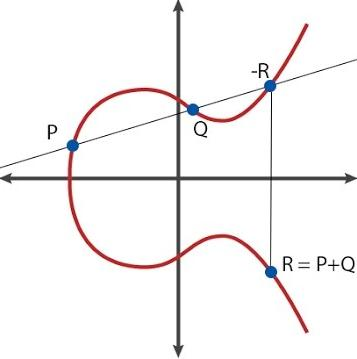
\includegraphics[scale=0.7]{pictures/hqdefault.jpg} 
\caption{vision graphique de l'addition de deux points sur la courbe}
\end{figure}



Maintenant que l'on dispose de formule d'additions pour deux points sur une courbe elliptique on peut donner un sens à la multiplication scalaire d'un point comme $kP = \underbrace{P + \ldots + P}_{k \text{ fois}}$. On va noter cette multiplication scalaire par :
\newline

$\begin{array}{ccccc}
[l]_E & : & E(\mathbb{K}) & \to & E(\mathbb{K}) \\
 & & P & \mapsto & lP\\
\end{array}$

Ce qui nous permet de définir l'ensemble des points de l-torsion comme le noyau de $[l]$. On note $E[l]$ cet ensemble.
\newline
$$E[l] = \left\{ P \in E(\overline{\mathbb{K}}) \, | \, [l]P = 0_E \right\} $$

\section{Compter les points sur une courbe}
On va considérer dans la suite que la caractéristique du corps utilisée pour définir nos courbes elliptiques est plus grande que $3$. On peut donc écrire notre courbe elliptique sur $\mathbb{F}_p$ sous leur forme réduite $y^2 = x^3 + ax+b$

\subsection{Algorithme naif}
On note $E: y^2 = f(x)$, compter les points de $E$ revient donc pour chaque valeur de $x \in \mathbb{F}_p$ à regarder si $f(x)$ est un carré modulo $p$. On calcule donc le symbole de Legendre de $f(x)$, on a les cas suivant : 
\begin{itemize}
\item  $\genfrac(){}{0}{f(x)}{p} = -1$, $f(x)$ n'est pas un carré modulo $p$, on ne trouve aucun point appartenant à la courbe.
\item $\genfrac(){}{0}{f(x)}{p} = 0$, $f(x)$ est divisible par $p$, on trouve $1$ point sur la courbe.
\item $\genfrac(){}{0}{f(x)}{p} = 1$, $f(x)$ est un carré modulo $p$, on trouve $2$ points sur la courbe.
\end{itemize}
\medskip
Au final en considérant le point à l'infini on peut calculer le nombre de points de $E$ : 
\begin{equation*}
\#E(\mathbb{F}_p) = 1 + \sum_{x \in \mathbb{F}_p}(\genfrac(){}{0}{f(x)}{p} + 1)
\end{equation*}
Soit : 
\begin{equation}
\#E(\mathbb{F}_p) = 1 + p +\sum_{x \in \mathbb{F}_p}\genfrac(){}{0}{f(x)}{p}
\end{equation}
La complexité est en la taille de $p$. Cette méthode est pratique quand $p$ est petit mais devient impraticable s'il est trop grand. On illustre ce fait par un algorithme simple :
\medskip
\begin{lstlisting}
def brute_force(p, a,b):
    R.<x> = PolynomialRing(GF(p))
    f = x**3 + a*x + b
    return 1+p+sum([kronecker(f(i),p) for i in range(p)])

\end{lstlisting}

On va tester la non efficacité de cette méthode lorsque $p$ devient trop grand par le graphique suivant:

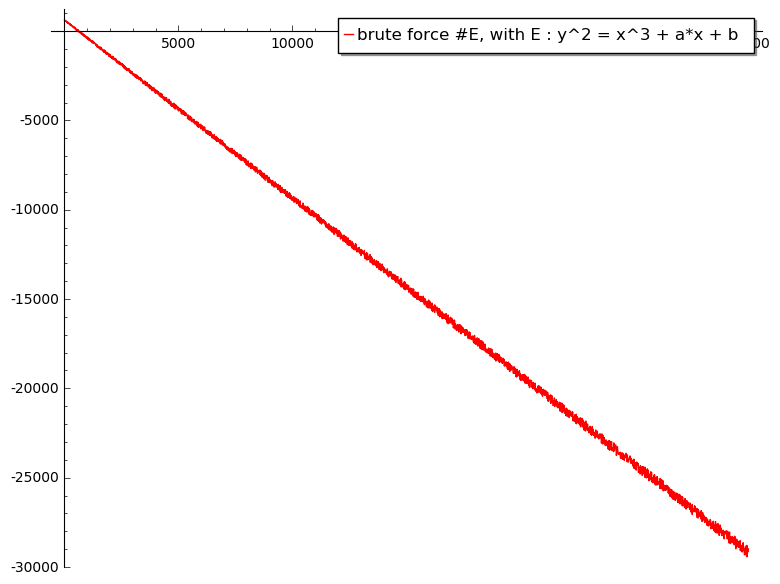
\includegraphics[scale=0.5]{pictures/brute_force_cputime.png} 

On retrouve bien l'aspect linéaire en $p$ évoqué précédemment.
\subsection{Shanks}
Il s'agit d'un algorithme Baby steps-giant steps de complexité exponentielle.

\subsection{Schoof}
Soit $E$ une courbe elliptique défini sur $\mathbb{F}_p$ avec $p$ premier $>3$ sous sa forme réduite 
$$ E: y^2 = x^3 + ax+b$$
On rappelle le théorème de Hasse-Weil:

\begin{thm}
$\#E(\mathbb{F}_p) = p + 1 - t$ avec $|t| \leq 2 \sqrt{p}$ trace de l'endomorphisme de Frobenius de $E$.
\end{thm}
Pour trouver le nombre de points de $E$ il faut donc déterminer $t$. 
L'idée de Schoof est de calculer $t$ modulo de petits nombres premiers puis d'utiliser le théorème des restes chinois. 

Avant de développer l'algorithme il est nécessaire de donner d'autres définitions. 

\begin{defi}[Frobenius]
Soit $E$ une courbe elliptique défini sur $\mathbb{F}_p$, l'endomorphisme de Frobenius est défini par 

$\begin{array}{ccccc}
\phi_p & : & E(\mathbb{F}_p) & \to & E(\mathbb{F}_p) \\
 & & (x,y) & \mapsto & (x^p, y^p) \\
\end{array}$
\end{defi}
On peut définir le polynôme caractéristique de cet endomorphisme par $\phi_p^2 - t \phi_p + p = 0$, cette relation reste en particulier vrai sur les points de $l$-torsion, ce qui nous sera utile par la suite. Ainsi nous avons : 
\begin{equation}
\label{eqnfrobenius}
 \phi_p^2(P)  + [p_l]P = [t_{l}] \phi_p(P) \quad \forall P \in E[l]
\end{equation} 
Avec $t_l \equiv t \pmod l$, $p_l \equiv p \pmod l$ et $0 \leq t_l, p_l \leq l$. 
\newline
Il faut aussi introduire les polynôme de division d'une courbe elliptiques $E$.

\begin{defi}
Soit une courbe elliptique $E : y^2 = x^3 + ax+b$ défini sur $\mathbb{K}$. On appelle $f_n(X)$ le n-ième polynôme de divisons définit sur $\mathbb{Z}[x]$ de manière récursive par : 


\begin{align*}
f_0(x) &= 0 \\
f_1(x) &= 1 \\
f_2(x) &= 1 \\
f_3(x) &= 3x^4 + 6ax^2 +12bx - a^2 \\
f_4(x) &= 2x^6 + 10ax^4 +40bx^3 - 10a^2x^2 - 8abx - 2(a^3 + 8b^2)
\end{align*}
On pose $F(X)= 4x^3 + 4ax + 4b$, et on a:

\begin{equation}
\left\lbrace
\begin{array}{ll}
f_{2n}& =  f_n(f_{n+2}f_{n-1}^2 - f_{n-2}f_{n+1}^2)   \\
f_{2n+1}& = \left\lbrace 
\begin{array}{ccc}
F^2f_{n+2}f_n^3 - f_{n-1}f_{n+1}^3 & \mbox{si} & n \text{ est pair}\\
f_{n+2}f_n^3 - f_{n-1}f_{n+1}^3F^2 & \mbox{si} & n \text{ est impair} \end{array}\right.

\end{array} \right.
\end{equation} 
Ces polynômes sont de degrés au plus $\frac{(n^2 -1)}{2}$ si $n$ est pair, ou bien  au plus $\frac{(n^2 -2)}{2}$ si $n$ est impair.
\end{defi}

\begin{proof}
Preuve du degré de $f_n$ ? 
Avec $n$ premier on a $E[n] \simeq \frac{\mathbb{Z}}{n\mathbb{Z}} \times \frac{\mathbb{Z}}{n\mathbb{Z}}$, soit $n^2 - 1$ points de n-torsion ? on doit les compter 2 fois donc j'imagine. Sinon la démo doit découler toute seule en utilisant les formules de recurrence mais un peu plus pénible a écrire
\end{proof}

On peut utiliser les polynôme de division pour calculer la multiplication scalaire d'un point de la courbe $E$.
On a les formules suivantes : 

\begin{thm}
Soit $E$ une courbe elliptique défini sur $\mathbb{K}$, un point $P$ sur cette courbe et $m \in \mathbb{N}^*$.

\begin{equation}
[m]P = 
\left\lbrace
\begin{array}{ccc}
O_E & \mbox{si} & P \in E[m]  \\
\left(    \frac{\phi_m(x,y)}{\psi^2_m(x,y)}, \frac{\omega_m(x,y)}{\psi^3_m(x,y)}\right) & \mbox{sinon}  & 
\end{array}\right.
\end{equation}

En posant : 
\begin{equation*}
\psi_m= \left\lbrace
\begin{array}{cc}
2yf_m & \mbox{si m est pair} \\
f_m & \mbox{sinon}
\end{array}\right.
\end{equation*}
et 
\begin{equation*}
\left\lbrace
\begin{array}{ll}
\phi_m &= x \psi^2_m - \psi_{m-1}\psi_{m+1} \\
\psi_m \omega_m &= \psi_{2m}
\end{array}\right.
\end{equation*}
On peut aussi réécrire $[m]P$ sous cette forme : 
\begin{equation}\label{mP}
[m]P = \left\lbrace
\begin{array}{lll}
O_E & \mbox{si} & P \in E[m]  \\
\left(  X -   \frac{\psi_{m-1}(x,y)\psi_{m+1}(x,y)}{\psi^2_m(x,y)}, \frac{\psi_{2m}(x,y)}{\psi^4_m(x,y)}\right) & \mbox{sinon}  & 
\end{array}\right.
\end{equation}
\end{thm}

\begin{proof}
On veut démontrer \ref{mP}. 
\newline
On note $[m]P = (x_1, y_1)$ 
On a alors : 

\begin{align*}
y_1 &= \frac{\omega_m}{\psi^3_m} = \frac{\psi_{2m}}{\psi_m} \frac{1}{\psi_m^3} = \frac{\psi_{2m}}{\psi_m^4} \\
x_1 &= \frac{\phi_m}{\psi^2_m} =  \frac{X \psi^2_m - \psi_{m-1}\psi_{m+1}}{\psi_m^2} = X - \frac{\psi_{m-1}\psi_{m+1}}{\psi_m^2}	
\end{align*}




\end{proof}
On remarque que $[m]P = (x_1, y_1)$ avec $x_1$ uniquement fonction de $x$. En effet en utilisant les formules de récurrence, si $m$ est pair $\psi_m^2 = 4y^2f_m$, mais en utilisant l'équation de $E$ on peut remplacer $y^2$ par une fonction de $x$, et les polynômes de division sont en fonction de $x$. De plus comme $m$ est pair les polynômes $\psi_{m+1} et \psi_{m-1}$ sont uniquement en fonction de $x$. Dans le cas où $m$ est impair on à l'inverse, le numérateur fait apparaître un $y^2$ qu'on peut remplacer par une fonction de $x$ comme précédemment et le dénominateur est une fonction de $x$. Quand à $y_1$, son degré en $y$ est au plus $1$. Si $m$ est pair $\psi_m^4$ fait apparaître un $y^4$ qui s'exprime en fonction de $x$, et $\psi_{2m}$ amène un $y$. On montre la même chose quelque soit la parité de $m$ et $2m$.
On peut ainsi exprimer $[m]P$ comme un polynôme en $X,Y$. Mais ce n'est pas la seule particularité de ces polynôme utile pour notre algorithme. En effet $P = (x_1, y_1)$ est un point de l-torsion si et seulement si $x_1$ est une racine du l-ième polynôme de division $f_l$. De plus $P$ est sur la courbe $E$. Les points de l-torsion sont donc solution du système d'équation : 
\begin{equation}
E(x,y) = y^2 - x^3 - ax - b = 0, \quad f_l(x) = 0
\end{equation}
L'équation \ref{eqnfrobenius} peut donc se réécrire en utilisant les points de l-torsion. On va maintenant faire des calculs dans l'anneau $\mathbb{W}= \frac{\mathbb{F_p}[x,y]}{(f_l(x), E(x,y))}$.L'idée de l'algorithme de Schoof est donc de tester pour des valeurs $\tau_l \in \lbrace 0, \ldots, l-1 \rbrace$ si l'équation suivante est vrai dans cet anneau :

\begin{equation}
(x^{p^2}, y^{p^2}) + [p_l](x,y) = [\tau_l](x^{p}, y^{p})  \quad, P=(x,y)
\end{equation}
L'unique solution que l'on trouve est $t_l$.On répète l'opération pour d'autres $l$ premiers jusqu'à avoir assez de $t_l$ pour appliquer le théorème des restes chinois et retrouver la valeur de $t$. L’intérêt de travailler avec des points de $l$-torsion est ainsi de pouvoir borner la taille des polynômes en jeu dans l'équation du Frobenius, en $O(l^2)$, ce qui est plus efficace qu'uniquement travailler avec des fonctions rationnelles.
\newline
\medskip
On va maintenant détailler l'algorithme étape par étape. 


\subsubsection{Choix de l'ensemble de premiers}
L'idée de Schoof est de calculer la trace de l'endomorphisme de Frobenius modulo de petits premiers. Il faut choisir un ensemble $S = (l_1, \ldots l_n)$ tel que $\prod l_i > 4\sqrt{p}$. En effet on rappelle que  $|t| \leq 2 \sqrt{p}$, on veut s'assurer de bien pouvoir reconstruire notre solution quand on va utiliser les restes chinois. Pour construire $S$ on va juste ajouter des nombres premiers à une liste en utlisant la fonction \path{next_prime} de SAGE tant que le produit des éléments de $S$ est plus petit que $ 4\sqrt{p}$.



\subsubsection{Cas $l=2$}
Ce cas est particulier et doit être traiter à part car on suppose nos premiers impairs. 0n a $t_2 \equiv 0 \pmod 2$ si et seulement si $E(\mathbb{F_p})$ à un élément d'ordre $2$, c'est à dire un point de $2$-torsion. Or les points de $2$ torsions sont de la forme $(x, 0)$. En effet, si $2P = 0$, pour $P \in E(\mathbb{F_p})$ alors $P = -P$, et cela correspond aux points de l'axe des abscisses. Ainsi $t_2$ est congru à $0$ si et seulement si $x^3 +ax +b$ à une racine dans $\mathbb{F_p}$. Mais les racines de $\mathbb{F_p}$ sont entièrement déterminé par le polynôme $x^p - x$, nos deux polynômes partageraient alors une racine commune. La façon utilisé ici pour décider si $t_2 \equiv 0 \pmod 2$ est donc de calculer si $\gcd(x^p - x, x^3 +ax +b) \ne 1$.

\subsubsection{Calcul des polynômes de division}
Il existe dans SAGE une fonction permettant de calculer les polynôme de division, \path{polynomial_polynomial(n)} renvoyant le n-ième polynôme de division. Mais comme au cours de l'algorithme on doit souvent utiliser différents polynôme de division et de plus ils sont calculé via des formules de récurrence. Il ne me paraissait pas forcement très judicieux d'utiliser la fonction de sage qui allait de toute façon très certainement à chaque appel devoir recalculer via les formules de récurrence le polynôme souhaité. L'idée étant de stocker tous ces polynômes dans un dictionnaire, une fois la phase de pré calcul faite on peut donc accéder à tous les polynômes de division que l'on souhaite en temps constant au cours de l’exécution de l'algorithme de Schoof. Et en utilisant la fonction de SAGE j'ai tout de même vérifié via une fonction de test que je trouvais bien les même polynômes qu'avec ma fonction.


\subsubsection{Calcul de $(x^{p^2}, y^{p^2}) + [p_l](x,y)$}

Comme vu en introduction aux courbes elliptiques la somme de deux points appartenant à la courbe dépend de plusieurs cas. Est ce que nos points sont distincts où ont la même coordonnée en $x$. En effet les formules à appliquer seront différentes dépendamment que l'on soit dans un cas ou l'autre. Il est plus probable d'avoir des coordonnées différentes, on va donc travailler dans ce cas la. Si l'algorithme trouve un $t_l$ vérifiant l'équation on est dans le bon cas, s'il n'en trouve aucun cela veut dire que l'on se trouve dans l'autre cas.
\paragraph*{Cas : $(x^{p^2}, y^{p^2}) \ne \pm [p_l](x,y)$}

On peut utiliser notre formule usuelle d'addition sur courbe elliptique pour calculer $(x_1, y_1) = (x^{p^2}, y^{p^2}) + (x_{\bar{p_l}}, Y_{\bar{p_l}})$ en notant $(x_{\bar{p_l}}, y_{\bar{p_l}}) =  [p_l](x,y)$. 
\newline
Soit $\lambda = \frac{y_{\bar{p_l}} - y^{p^2}}{x_{\bar{p_l} - x^{p^2}}}$, on a alors :
\begin{equation}
(x_1, y_1) = (\lambda^2 - x^{p^2} - x_{\bar{p_l}}, \, \lambda (x^{p^2} - x_1) -  y^{p^2})
\end{equation}
On va aussi noter $(x_{\tau}, y_{\tau}) =  [\tau](x,y)$. On doit maintenant tester en faisant varier la valeur de $\tau$ entre $0$ et $l -1$ si $x_1 = x_{\tau}$. Si c'est le cas on se retrouve avec deux possibilités comme valeur de $y_1$, soit on a le point soit on a son opposé. On regarde donc si $y_1 = y_{\tau}$, on a alors $t_l = \tau$, sinon on a $t_l = - \tau$

\paragraph*{Cas : $(x^{p^2}, y^{p^2}) = \pm [p_l](x,y)$}
La encore deux cas possible. On va d'abord regarder lorsque $(x^{p^2}, y^{p^2}) = [p_l](x,y)$. 
\newline
Soit $P=(x,y)$, on rappelle l’équation caractéristique de l'endomorphisme Frobenius restreinte aux points de $l$-torsion: 
\begin{equation}
\phi_p^2(P)  + [p_l]P = [t_{l}] \phi_p(P) \quad \pmod{l}
\end{equation}
On a alors dans notre cas $2[p_l]P = [t_{l}] \phi_p(P) \, \pmod{l}$. De plus on a $\phi_p^2 = [p_l]P$. En combinant ces deux égalités on trouve :

\begin{equation}
[t_l^2 p_l]P = [t_l^2] \phi_p^2 = [t_l] \phi ([t_l] \phi_p) = [(2p_l)^2]P \quad \pmod{l}
\end{equation}
Ainsi $p_l$ est un carré modulo $l$. On pose $p_l = \omega^2 \pmod{l}$. On va maintenant calculer $\omega \phi P$, si $[p_l]P = \omega \phi P$ alors $t_l = 2\omega$ sinon $t_l = -2\omega$.
\newline
\medskip
Si $p_l$ n'est pas un carré modulo $l$ on est dans le cas $(x^{p^2}, y^{p^2}) = - [p_l](x,y)$ et on on a alors $t_l = 0$ d'après l'équation caractéristique. 



\newpage
\paragraph{Algorithme}
On donne une version complète en langage naturel de l'algorithme de schoof : 

\begin{algorithm}
\caption{Schoof}
\begin{algorithmic}
\REQUIRE $E$ une courbe elliptique de la forme $y^2 = x^3 + ax = b$ sur $\mathbb{F}_p$
\ENSURE Le nombre de points de $E$

\STATE Choisir un ensemble de premier S tel que $\prod_{l \in S}l \leq 4\sqrt{p}$
\IF{$\gcd(x^q - x, x^3 + ax +b) \ne 1$} 
\STATE $t_2 = 0$
\ELSE
\STATE $t_2 = 1$
\ENDIF

\FORALL{$l \in S$}
\STATE Calculer le polynôme de division $f_l$, on fera les calculs dans l'anneau $\mathbb{F}= \frac{\mathbb{F_p}[X,Y]}{(f_l(X), y^2 -x^3 - ax - b})$
\STATE On pose $p_l = p \mod(l)$
\STATE Calculer $(x^p, y^p), \, (x^{p^2}, y^{p^2}), \, [p_l](x, y) = (x_{p_l}, y_{p_l})$
\IF{$x^{p^2} \ne  x_{p_l}$}
\STATE Calculer $(X, Y) = (x^{p^2}, y^{p^2}) + (x_{p_l}, y_{p_l})$
\FORALL{$1 \leq \tau \leq l - 1$}
\IF{$X = x^p_{\tau}$}
\IF{$Y = y^q_{p_l}$}
\STATE $t_l = \tau$
\ELSE 
\STATE $t_l = - \tau$
\ENDIF
\ENDIF
\ENDFOR
\ELSE
\IF{$p$ est un carré modulo $l$}
\STATE Calculer $w$ tel que $p \equiv w^2 \pmod l$ 
\STATE Calculer $[w](x^p,y^p)]$
\IF{$[w](x^p,y^p)] = (x^{p^2}, y^{p^2})$}
\STATE $t_l = 2w$
\ENDIF
\IF{$[w](x^p,y^p)] = (x^{p^2}, -y^{p^2})$}
\STATE $t_l = -2w$
\ELSE
\STATE $t_l =0$
\ENDIF
\ELSE
\STATE $t_l = 0$

\ENDIF
\ENDIF
\ENDFOR
\end{algorithmic}
\end{algorithm}


\subsubsection{Exemple}
On va travailler avec la courbe $E$ suivante, $E$ : $y^2 =x^3 +2x+1$ sur $\mathbb{F}_{19}$.

\paragraph{$\textbf{l=2}$}
On calcule $\gcd(x^{19} -x, x^3 + 2x+1)$ et on trouve $1$, donc $t \equiv 1 \pmod 2$

\paragraph{$\textbf{l=3}$}
On a $p^2 = 361$ et $p_l \equiv 1 \pmod 3$, on pose ainsi $p_l = 1$. L'équation du Frobenius devient : 
\begin{equation}
(x^{361}, y^{361}) + (x,y) = [\tau_l](x^{19}, y^{19})  \quad (x,y) \in E[3], \, \tau_l = \pm 1
\end{equation}
Le troisième polynôme de division est $f_l = 3x^4 + 12x^2 +12x - 4$ mais ce polynôme n'est pas irréductible dans $\mathbb{F}_{19}$, on va plutôt travailler avec un de ces diviseurs : $x^3 + 8x^2+16$.
\newline 
Il nous faut maintenant calculer la partie gauche de cette équation.
On a $x^{361} = 3x^2 +2x +5 \pmod f_{l}$ et $y^{361} = y(y^2)^{180} = y(4x^2+9x+16)$. On est dans le cas ou $x^{361} \ne x$. On doit maintenant utiliser nos formules de sommations pour calculer $(x_3, y_3) =(x^{361}, y^{361}) + (x,y)$ : 

\begin{align*}
x_3 &= (\frac{y(4x^2+9x+16) - y}{3x^2 +2x +5 - x})^2 -3x^2 -2x - 5 - x 
 	&= (y(4x^2+9x+15)(x^2+15x+6))^2 -3x^2 -3x - 5 \\
 	&= 11 - 3x^2 -3x - 5  \\
 	&= 16x^2 + 16x + 6 
\end{align*}
et, 

\begin{align*}
y_3 &= \frac{y(4x^2+9x+16) - y}{3x^2 +2x +5 - x} (4x^2+9x+16 -  16x^2 - 16x - 6) - y(4x^2+9x+16) \\
	&= y(4x^2+9x+15)(x^2+15x+6)( -12x^2 - 7x +10 ) - y(4x^2+9x+16)\\
	&= y(13x^2 + 13x + 14)
\end{align*}
(reprendre le calcul de $y_3$, le resultat final est juste mais erreur dans les calcules intermédiaire !

Maintenant nous devons calculer pour $\tau$ variant de $0$ à $2$ si $(x_3, y_3) = \tau (x^p, y^p)$.
\subsubsection{Complexité}
La complexité de l'algorithme de Schoof est en $O(\log{q}^8)$. L'algorithme est plus efficace qu'une version naive quand la taille de $p$ augmente mais reste néanmoins limité pour $p$ trop grand. En effet le degré des polynômes de division en $O(l^2)$ empêche une performance optimale pour des tailles de $p$ trop importante.Une solution est donc de travailler avec des polynômes plus adapté, de plus petit degré. 
\end{document}